% ============================================================================
% CausalShield — IEEE Format Research Paper (v2)
% Overleaf-Ready: All figures use TikZ/pgfplots (no external images needed)
% Compile with: pdfLaTeX
% ============================================================================
\documentclass[conference]{IEEEtran}

% ── Core Packages ────────────────────────────────────────────────────────────
\usepackage{cite}
\usepackage{amsmath,amssymb,amsfonts}
\usepackage{algorithmic}
\usepackage{algorithm}
\usepackage{graphicx}
\usepackage{textcomp}
\usepackage{xcolor}
\usepackage{booktabs}
\usepackage{multirow}
\usepackage{hyperref}
\usepackage{balance}
\usepackage{subcaption}
\usepackage{array}
\usepackage{colortbl}
\usepackage{enumitem}

% ── TikZ & pgfplots for figures ─────────────────────────────────────────────
\usepackage{tikz}
\usepackage{pgfplots}
\pgfplotsset{compat=1.18}
\usetikzlibrary{shapes.geometric, arrows.meta, positioning, calc, backgrounds, fit, decorations.pathreplacing}

% ── Colors ───────────────────────────────────────────────────────────────────
\definecolor{layer1}{HTML}{4A90D9}
\definecolor{layer2}{HTML}{E74C3C}
\definecolor{layer3}{HTML}{F39C12}
\definecolor{layer4}{HTML}{27AE60}
\definecolor{fragile}{HTML}{E74C3C}
\definecolor{robust}{HTML}{27AE60}
\definecolor{uncertain}{HTML}{F39C12}
\definecolor{protected}{HTML}{8E44AD}
\definecolor{lightblue}{HTML}{EBF5FB}
\definecolor{lightred}{HTML}{FDEDEC}
\definecolor{lightgreen}{HTML}{EAFAF1}
\definecolor{lightyellow}{HTML}{FEF9E7}
\definecolor{darkblue}{HTML}{1B4F72}

\hypersetup{
    colorlinks=true,
    linkcolor=darkblue,
    citecolor=darkblue,
    urlcolor=blue
}

\def\BibTeX{{\rm B\kern-.05em{\sc i\kern-.025em b}\kern-.08em
    T\kern-.1667em\lower.7ex\hbox{E}\kern-.125emX}}

\begin{document}

% ══════════════════════════════════════════════════════════════════════════════
% TITLE & AUTHORS
% ══════════════════════════════════════════════════════════════════════════════
\title{CausalShield: A Doubly Robust Causal Auditing\\Framework for Safe Explainability in Clinical\\Decision Support Systems}

\author{
\begin{minipage}[t]{0.3\textwidth}
\centering
\textbf{Avula Sesha Sai Chand}\\
\textit{Dept. of Computer Science \& Eng.}\\
\textit{IIIT Sri City}\\
Sri City, India\\
seshasaichand.a23@iiits.in
\end{minipage}
\hfill
\begin{minipage}[t]{0.3\textwidth}
\centering
\textbf{Vuppala Sai Naman}\\
\textit{Dept. of Computer Science \& Eng.}\\
\textit{IIIT Sri City}\\
Sri City, India\\
sainaman.v23@iiits.in
\end{minipage}
\hfill
\begin{minipage}[t]{0.3\textwidth}
\centering
\textbf{Draksharapu Sai Nitin}\\
\textit{Dept. of Computer Science \& Eng.}\\
\textit{IIIT Sri City}\\
Sri City, India\\
sainitin.d23@iiits.in
\end{minipage}
}

\maketitle

% ══════════════════════════════════════════════════════════════════════════════
% ABSTRACT
% ══════════════════════════════════════════════════════════════════════════════
\begin{abstract}
Clinical AI models for hospital readmission prediction increasingly rely on post-hoc explanation methods such as SHAP and LIME. However, these methods expose only \textit{correlational} feature importance, creating a critical patient safety problem: a model may flag insulin as a top risk factor not because insulin causes readmission, but because sicker patients receive it --- a classic case of \textit{confounding by indication}. We propose \textbf{CausalShield}, a four-layer framework that transforms correlational explanations into causally-validated, clinically safe recommendations. Operating on the UCI Diabetes 130-US Hospitals dataset (101,766 encounters), the pipeline integrates: (1)~Gradient Boosted Trees for prediction, (2)~SHAP for associative explanation, (3)~Doubly Robust Estimation (DoubleML/AIPW) with E-value sensitivity analysis for causal auditing, and (4)~counterfactual recourse constrained to causally-validated features. Results show that 7 of 10 top SHAP features are causally fragile ($E < 2.0$), while discharge disposition ($E = 4.10$) and HbA1c ($E = 3.21$) are robust. The framework blocks dangerous recommendations like ``reduce insulin'' and generates safe, actionable clinical guidance. To our knowledge, this is the first system integrating SHAP, doubly robust causal estimation, E-value analysis, and causally-constrained counterfactuals into a unified clinical AI auditing pipeline.
\end{abstract}

\begin{IEEEkeywords}
Explainable AI, Causal Inference, SHAP, Double Machine Learning, CATE, Counterfactual Explanations, Clinical Decision Support, Hospital Readmission, Confounding by Indication, E-values
\end{IEEEkeywords}

% ══════════════════════════════════════════════════════════════════════════════
% I. INTRODUCTION
% ══════════════════════════════════════════════════════════════════════════════
\section{Introduction}

Artificial Intelligence is reshaping clinical medicine. The 30-day hospital readmission metric alone costs the US healthcare system \$26 billion annually~\cite{cms2023readmission}, making accurate AI-driven risk prediction of significant clinical and economic value. However, deploying AI in clinical settings demands more than accuracy --- physicians need to understand \textit{why} a model flags a patient as high-risk.

This has driven the adoption of eXplainable AI (XAI) methods such as SHAP~\cite{lundberg2020local} and LIME~\cite{ribeiro2016lime}. Yet these tools reveal only statistical \textit{associations}, not causal drivers. In clinical medicine, this distinction is a patient safety issue.

\subsection{Motivating Example: The Insulin Paradox}

Consider a readmission model where SHAP assigns insulin a high positive importance score ($+0.12$), suggesting insulin \textit{increases} risk. A na\"ive interpretation could lead to dangerous insulin reduction. The reality is illustrated in Fig.~\ref{fig:dag}: doctors prescribe insulin to the \textit{sickest} patients, who are also readmitted more. The model has learned a spurious correlation through \textit{confounding by indication}~\cite{feuerriegel2024causal}.

% ── FIGURE 1: Causal DAG ────────────────────────────────────────────────────
\begin{figure}[htbp]
\centering
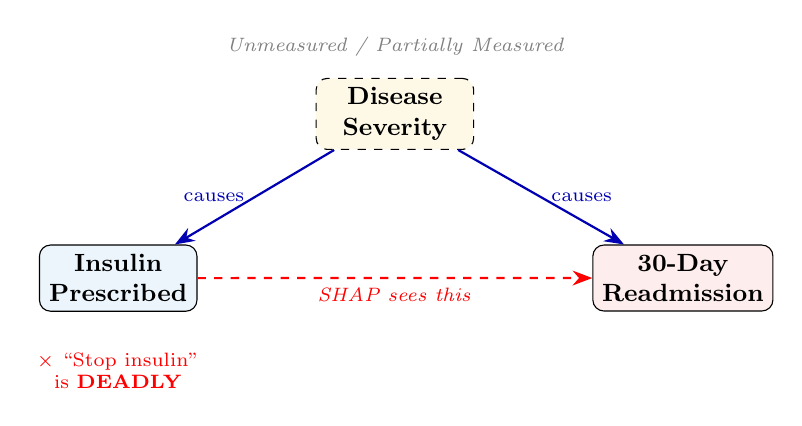
\begin{tikzpicture}[
    node distance=1.8cm and 2.5cm,
    every node/.style={font=\small},
    cause/.style={draw, rounded corners, fill=lightblue, minimum width=2cm, minimum height=0.7cm, align=center, font=\small\bfseries},
    effect/.style={draw, rounded corners, fill=lightred, minimum width=2cm, minimum height=0.7cm, align=center, font=\small\bfseries},
    hidden/.style={draw, dashed, rounded corners, fill=lightyellow, minimum width=2cm, minimum height=0.7cm, align=center, font=\small\bfseries},
    arr/.style={-{Stealth[length=2.5mm]}, thick},
    sarr/.style={-{Stealth[length=2.5mm]}, thick, red, dashed},
]
    % Nodes
    \node[hidden] (sev) {Disease\\Severity};
    \node[cause, below left=1.2cm and 1.5cm of sev] (ins) {Insulin\\Prescribed};
    \node[effect, below right=1.2cm and 1.5cm of sev] (read) {30-Day\\Readmission};

    % True causal arrows
    \draw[arr, blue!70!black] (sev) -- node[left, font=\scriptsize, text=blue!70!black] {causes} (ins);
    \draw[arr, blue!70!black] (sev) -- node[right, font=\scriptsize, text=blue!70!black] {causes} (read);

    % Spurious arrow (what SHAP sees)
    \draw[sarr] (ins) -- node[below, font=\scriptsize, text=red] {\textit{SHAP sees this}} (read);

    % Labels
    \node[above=0.15cm of sev, font=\scriptsize\itshape, text=gray] {Unmeasured / Partially Measured};
    \node[below=0.4cm of ins, font=\scriptsize, text=red, align=center] {$\times$ ``Stop insulin''\\is \textbf{DEADLY}};
\end{tikzpicture}
\caption{Causal DAG illustrating confounding by indication. Disease severity causes \textit{both} insulin prescription and readmission. SHAP incorrectly attributes the readmission association to insulin itself (red dashed arrow).}
\label{fig:dag}
\end{figure}

\subsection{Research Gap}
Despite extensive literature on XAI, causal inference, and counterfactual explanations \textit{separately}, no published framework integrates all four components --- prediction, explanation, causal audit with robustness quantification, and causally-constrained recourse --- into a unified pipeline.

\subsection{Contributions}
\begin{enumerate}[leftmargin=*, nosep]
    \item \textbf{End-to-end Causal Audit Framework:} First pipeline integrating SHAP, DoubleML/AIPW, E-values, and safe counterfactual recourse.
    \item \textbf{Empirical confounding detection:} 70\% of top SHAP features proven causally fragile on 101K real clinical records.
    \item \textbf{Causally-safe recourse:} Dangerous recommendations (e.g., ``reduce insulin'') are automatically blocked.
    \item \textbf{E-value as recourse filter:} Novel use of sensitivity analysis for feature selection in counterfactual generation.
    \item \textbf{Fairness integration:} Disparate impact analysis across age, race, and gender.
    \item \textbf{Open-source clinical dashboard:} Interactive Streamlit UI for real-time patient assessment.
\end{enumerate}

% ══════════════════════════════════════════════════════════════════════════════
% II. RELATED WORK
% ══════════════════════════════════════════════════════════════════════════════
\section{Related Work}

Table~\ref{tab:related} summarizes the key related works and their relationship to CausalShield.

\begin{table*}[htbp]
\caption{Summary of Related Work and Their Role in CausalShield}
\centering
\footnotesize
\renewcommand{\arraystretch}{1.2}
\begin{tabular}{p{3.5cm}p{2.2cm}p{4.5cm}p{3.5cm}p{2cm}}
\toprule
\textbf{Paper} & \textbf{Venue} & \textbf{Key Contribution} & \textbf{Limitation} & \textbf{Our Layer} \\
\midrule
Lundberg et al. (2020)~\cite{lundberg2020local} & Nature MI & TreeExplainer: exact Shapley values for trees & Correlation only, not causation & Layer 1--2 \\
Wachter et al. (2017)~\cite{wachter2017counterfactual} & Harvard JLT & Counterfactual explanations for GDPR compliance & No causal/correlational distinction & Layer 4 \\
Feuerriegel et al. (2024)~\cite{feuerriegel2024causal} & Nature Medicine & CATE estimation for clinical treatment effects & Framework only, no XAI integration & Layer 3 \\
Carloni et al. (2025)~\cite{carloni2025causality} & WIREs DMKD & Systematic review: causality $\times$ XAI & Survey, no implementation & Theoretical \\
Fernandez-Loria et al. (2022)~\cite{fernandez2022explaining} & MIS Quarterly & Decision-focused (not prediction-focused) CFEs & No causal validation of features & Layer 4 \\
Bienefeld et al. (2023)~\cite{bienefeld2023solving} & npj Digital Med & Clinical trust requires plausible explanations & Single hospital, no causal audit & Dashboard \\
\midrule
\textbf{CausalShield (Ours)} & --- & \textbf{End-to-end: SHAP + DoubleML + E-values + Safe CFEs} & \textbf{See Sec. VII} & \textbf{All layers} \\
\bottomrule
\end{tabular}
\label{tab:related}
\end{table*}

\textbf{SHAP and TreeExplainer.} Lundberg et al.~\cite{lundberg2020local} introduced polynomial-time exact Shapley value computation for tree models. While enabling real-time clinical deployment, SHAP values reflect \textit{model reliance}, not \textit{causal effect}. High SHAP values may arise entirely from confounding.

\textbf{Counterfactual Explanations.} Wachter et al.~\cite{wachter2017counterfactual} proposed counterfactuals as GDPR-compliant explanations: ``\textit{If X had been Y, the decision would have been Z}.'' Their $L_1$-norm minimization finds sparse changes but does not distinguish causal from correlational changes --- a gap we address.

\textbf{Causal ML in Medicine.} Feuerriegel et al.~\cite{feuerriegel2024causal} formalized confounding by indication and advocated CATE estimation under unconfoundedness and positivity assumptions. Their framework provides the theoretical foundation for our Layer~3.

\textbf{Causality $\times$ XAI.} Carloni et al.~\cite{carloni2025causality} reviewed 51 papers identifying three perspectives: Critics (XAI lacks causal grounding), XAI-for-Causality (hypothesis generation), and Causality-for-XAI (the most promising direction). Our work operationalizes the third perspective.

\textbf{Decision-Focused CFEs.} Fernandez-Loria et al.~\cite{fernandez2022explaining} showed that SHAP/LIME fail to identify \textit{decision-flipping} features. Valid explanations must pass their ``change test'' --- modifying the feature must flip the decision. This informs our counterfactual layer.

% ══════════════════════════════════════════════════════════════════════════════
% III. PROPOSED METHODOLOGY
% ══════════════════════════════════════════════════════════════════════════════
\section{Proposed Methodology}

The \textbf{Causal-Audit Decision Support System (CA-DSS)} is a four-layer sequential pipeline. Fig.~\ref{fig:arch} illustrates the complete architecture.

% ── FIGURE 2: Architecture ──────────────────────────────────────────────────
\begin{figure*}[htbp]
\centering
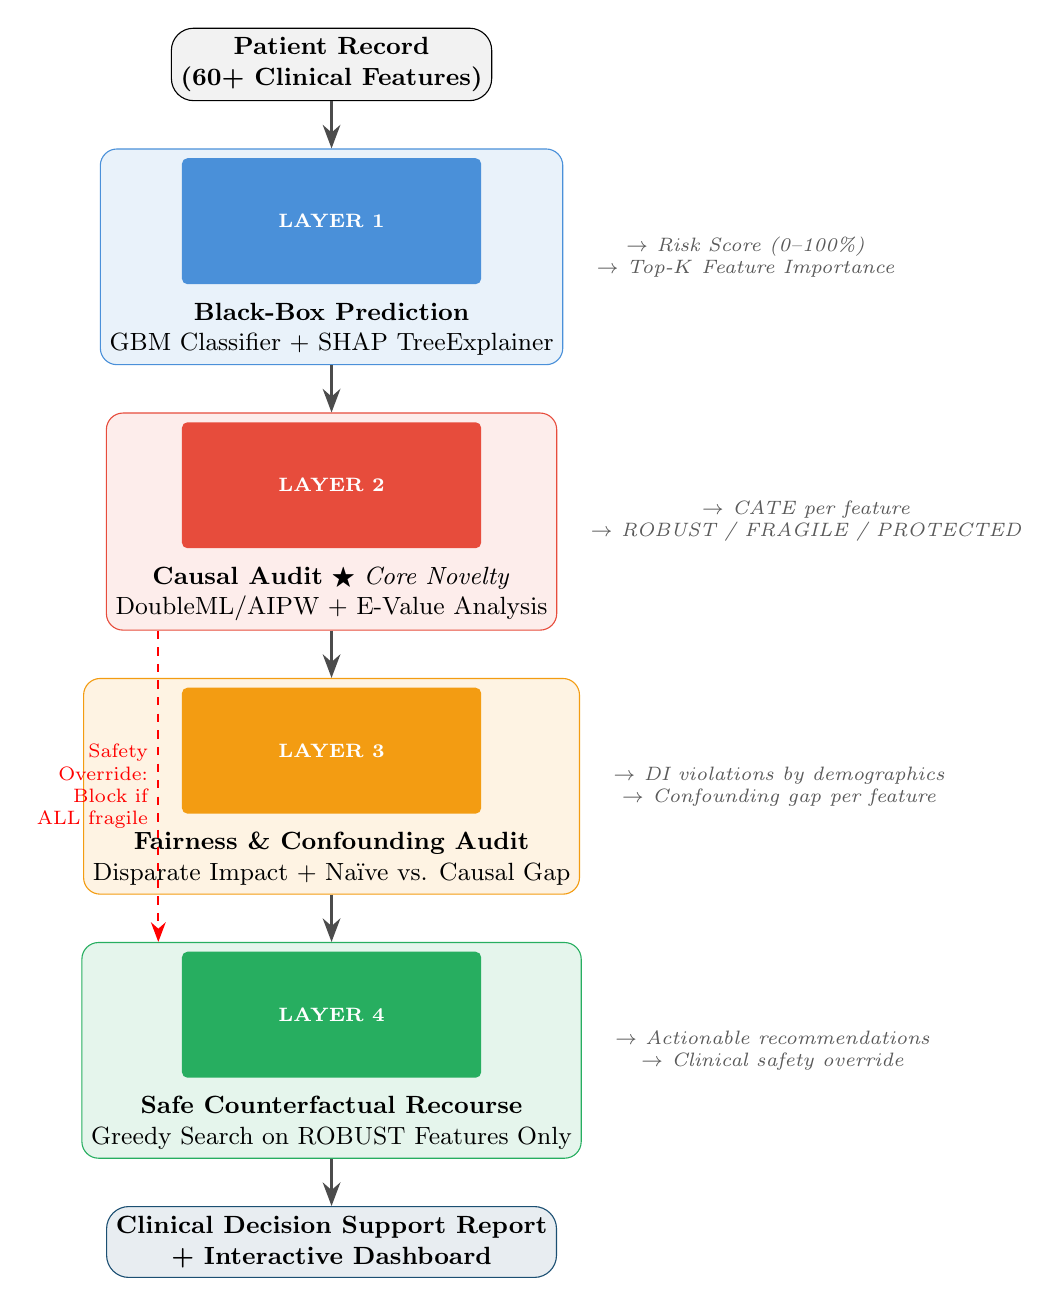
\begin{tikzpicture}[
    node distance=0.4cm,
    every node/.style={font=\small},
    input/.style={draw, rounded corners=8pt, fill=gray!10, minimum width=3.8cm, minimum height=0.9cm, align=center, font=\small\bfseries},
    layer/.style={draw, rounded corners=6pt, minimum width=3.8cm, minimum height=1.6cm, align=center, font=\small},
    output/.style={draw=none, minimum width=3.8cm, minimum height=0.6cm, align=center, font=\scriptsize\itshape, text=gray!70!black},
    arr/.style={-{Stealth[length=3mm]}, thick, gray!60!black},
    label/.style={font=\scriptsize\bfseries, text=white, fill=#1, rounded corners=2pt, inner sep=2pt},
]
    % Input
    \node[input] (inp) {Patient Record\\(60+ Clinical Features)};

    % Layer 1
    \node[layer, fill=layer1!12, draw=layer1, below=0.6cm of inp] (l1) {
        \tikz\node[label=layer1]{LAYER 1};\\[2pt]
        \textbf{Black-Box Prediction}\\
        GBM Classifier + SHAP TreeExplainer
    };
    \node[output, right=0.3cm of l1] (o1) {$\rightarrow$ Risk Score (0--100\%)\\$\rightarrow$ Top-$K$ Feature Importance};

    % Layer 2
    \node[layer, fill=layer2!10, draw=layer2, below=0.6cm of l1] (l2) {
        \tikz\node[label=layer2]{LAYER 2};\\[2pt]
        \textbf{Causal Audit} $\bigstar$ \textit{Core Novelty}\\
        DoubleML/AIPW + E-Value Analysis
    };
    \node[output, right=0.3cm of l2] (o2) {$\rightarrow$ CATE per feature\\$\rightarrow$ ROBUST / FRAGILE / PROTECTED};

    % Layer 3
    \node[layer, fill=layer3!12, draw=layer3, below=0.6cm of l2] (l3) {
        \tikz\node[label=layer3]{LAYER 3};\\[2pt]
        \textbf{Fairness \& Confounding Audit}\\
        Disparate Impact + Na\"ive vs. Causal Gap
    };
    \node[output, right=0.3cm of l3] (o3) {$\rightarrow$ DI violations by demographics\\$\rightarrow$ Confounding gap per feature};

    % Layer 4
    \node[layer, fill=layer4!12, draw=layer4, below=0.6cm of l3] (l4) {
        \tikz\node[label=layer4]{LAYER 4};\\[2pt]
        \textbf{Safe Counterfactual Recourse}\\
        Greedy Search on ROBUST Features Only
    };
    \node[output, right=0.3cm of l4] (o4) {$\rightarrow$ Actionable recommendations\\$\rightarrow$ Clinical safety override};

    % Output
    \node[input, below=0.6cm of l4, fill=darkblue!10, draw=darkblue] (out) {Clinical Decision Support Report\\+ Interactive Dashboard};

    % Arrows
    \draw[arr] (inp) -- (l1);
    \draw[arr] (l1) -- (l2);
    \draw[arr] (l2) -- (l3);
    \draw[arr] (l3) -- (l4);
    \draw[arr] (l4) -- (out);

    % Safety override annotation
    \draw[thick, red, dashed, -{Stealth[length=2.5mm]}] ([xshift=-2.2cm]l2.south) -- ([xshift=-2.2cm]l4.north) node[midway, left, font=\scriptsize, text=red, align=right] {Safety\\Override:\\Block if\\ALL fragile};
\end{tikzpicture}
\caption{CausalShield four-layer architecture. Each layer feeds into the next. Layer~2 (Causal Audit) is the core novelty. A safety override path (red dashed) blocks all recommendations when every audited feature is classified as FRAGILE.}
\label{fig:arch}
\end{figure*}

\subsection{Layer 1: Prediction \& Associative Explanation}

\subsubsection{Gradient Boosted Trees (GBM)}
We employ a GBM classifier~\cite{chen2016xgboost} with $K=200$ trees, maximum depth 5, learning rate 0.1, and subsample rate 0.8. The model minimizes the regularized logistic loss:
\begin{equation}
\mathcal{L} = \sum_{i=1}^{n} \ell(y_i, \hat{y}_i) + \sum_{k=1}^{K} \left[\gamma T_k + \tfrac{1}{2}\lambda\|w_k\|^2\right]
\end{equation}
where $\ell$ is the logistic loss, $T_k$ is the number of leaves, and $w_k$ are leaf weights.

\subsubsection{SHAP TreeExplainer}
For patient $\mathbf{x}_i$, the prediction decomposes additively:
\begin{equation}
\hat{y}_i = \phi_0 + \sum_{j=1}^{p} \phi_j(\mathbf{x}_i)
\end{equation}
where $\phi_0$ is the baseline (population average) and $\phi_j$ is the Shapley value for feature $j$:
\begin{equation}
\phi_j = \!\!\sum_{S \subseteq F \setminus \{j\}} \!\!\frac{|S|!\,(|F|\!-\!|S|\!-\!1)!}{|F|!} \left[f_{S \cup \{j\}}(\mathbf{x}_i) - f_S(\mathbf{x}_i)\right]
\end{equation}

The top-$K$ features by mean absolute SHAP value ($K\!=\!7$) are selected for causal auditing.

\subsection{Layer 2: Causal Audit (Core Novelty)}

For each top SHAP feature, treated as binary treatment $T$, we estimate the Conditional Average Treatment Effect (CATE) using Doubly Robust (DR) estimation~\cite{chernozhukov2018doubleml}.

\subsubsection{Doubly Robust Estimation (AIPW)}
The AIPW estimator proceeds in three stages with 5-fold cross-fitting:

\textbf{Stage 1 (Propensity):} Random Forest Classifier estimates treatment probability $\hat{m}(\mathbf{X}_i) = \hat{P}(T\!=\!1 \mid \mathbf{X}_i)$, clipped to $[0.05, 0.95]$.

\textbf{Stage 2 (Outcome):} Separate RF Regressors for each treatment arm:
$\hat{g}_t(\mathbf{X}_i) = \hat{E}[Y \mid T\!=\!t, \mathbf{X}_i]$ for $t \in \{0, 1\}$.

\textbf{Stage 3 (DR Score):}
\begin{equation}
\hat{\psi}_i = \underbrace{(\hat{g}_1 - \hat{g}_0)}_{\text{outcome adj.}} + \underbrace{\frac{T_i(Y_i - \hat{g}_1)}{\hat{m}(\mathbf{X}_i)}}_{\text{treated corr.}} - \underbrace{\frac{(1\!-\!T_i)(Y_i - \hat{g}_0)}{1 - \hat{m}(\mathbf{X}_i)}}_{\text{untreated corr.}}
\label{eq:aipw}
\end{equation}

The CATE estimate is $\hat{\theta} = n^{-1}\sum_i \hat{\psi}_i$ with $\text{SE} = \text{std}(\hat{\psi})/\!\sqrt{n}$.

\textbf{Key property:} Eq.~\eqref{eq:aipw} is consistent if \textit{either} $\hat{m}$ or $\hat{g}$ is correctly specified --- hence ``doubly robust.''

\subsubsection{E-Value Sensitivity Analysis}
Following VanderWeele and Ding~\cite{vanderweele2017evalue}:
\begin{equation}
RR = \exp(\text{CI}_{\text{bound}}), \qquad E = RR + \sqrt{RR(RR - 1)}
\end{equation}
The E-value quantifies the minimum confounder strength needed to nullify the result. Features are classified per Table~\ref{tab:thresholds}.

\begin{table}[htbp]
\caption{Feature Classification by E-Value}
\centering
\renewcommand{\arraystretch}{1.1}
\begin{tabular}{>{\bfseries}l c l}
\toprule
\textbf{Status} & \textbf{E-Value} & \textbf{Recourse Action} \\
\midrule
\cellcolor{robust!15}ROBUST & $E > 3.0$ & \cellcolor{robust!15}Safe for recommendations \\
\cellcolor{uncertain!15}UNCERTAIN & $2.0 < E \leq 3.0$ & \cellcolor{uncertain!15}Flag for clinical review \\
\cellcolor{fragile!15}FRAGILE & $E \leq 2.0$ & \cellcolor{fragile!15}Exclude from recourse \\
\cellcolor{protected!15}PROTECTED & N/A & \cellcolor{protected!15}Immutable (demographic) \\
\bottomrule
\end{tabular}
\label{tab:thresholds}
\end{table}

\subsection{Layer 3: Fairness \& Confounding Audit}

\subsubsection{Disparate Impact Analysis}
For demographic group $g$, the disparate impact ratio is:
\begin{equation}
DI_g = \frac{P(\hat{Y}\!=\!1 \mid G\!=\!g)}{P(\hat{Y}\!=\!1 \mid G\!=\!g_{\text{ref}})}
\end{equation}
Groups with $DI < 0.80$ or $DI > 1.25$ are flagged~\cite{feldman2015fairness}.

\subsubsection{Na\"ive vs. Causal Gap}
A na\"ive logistic regression coefficient $\beta_j$ is compared to the DoubleML CATE. A large $|\beta_j \cdot \bar{p}(1\!-\!\bar{p}) - \text{CATE}_j|$ gap indicates confounding.

\subsection{Layer 4: Safe Counterfactual Recourse}

For high-risk patients ($P \geq 0.5$), we find minimum safe changes using Algorithm~\ref{alg:cf}.

\begin{algorithm}[htbp]
\caption{Safe Counterfactual Generation}
\label{alg:cf}
\begin{algorithmic}[1]
\REQUIRE Patient $\mathbf{x}$, model $f$, safe features $\mathcal{A}$, data $D$
\ENSURE Modified $\mathbf{x}'$, changes $C$
\STATE $\mathbf{x}' \leftarrow \mathbf{x}$; \ $C \leftarrow \emptyset$
\STATE Sort $\mathcal{A}$ by model importance (descending)
\FOR{$j \in \mathcal{A}$}
    \STATE $v^* \leftarrow \arg\min_{v \in \text{unique}(D_j)} f(\mathbf{x}'[j \leftarrow v])$
    \IF{$v^* \neq x'_j$}
        \STATE $x'_j \leftarrow v^*$; \ append $(j, x_j \to v^*)$ to $C$
    \ENDIF
    \IF{$f(\mathbf{x}') < 0.5$}
        \RETURN $\mathbf{x}', C$ \hfill $\triangleright$ \textit{Risk flipped}
    \ENDIF
\ENDFOR
\RETURN $\mathbf{x}', C$ \hfill $\triangleright$ \textit{Best effort}
\end{algorithmic}
\end{algorithm}

The safe feature set is $\mathcal{A} = \mathcal{A}_{\text{actionable}} \cup \{f : \text{Status}(f) = \text{ROBUST}\}$, containing 15 clinically actionable features (7 medications, 5 discharge types, 2 HbA1c indicators, 1 medication-change flag). All FRAGILE, PROTECTED, and immutable features are \textbf{hard-blocked}.

% ══════════════════════════════════════════════════════════════════════════════
% IV. DATASET AND EXPERIMENTAL SETUP
% ══════════════════════════════════════════════════════════════════════════════
\section{Dataset and Experimental Setup}

\subsection{Dataset Description}
We use the \textbf{UCI Diabetes 130-US Hospitals} dataset~\cite{strack2014impact}: 101,766 encounters from 130 US hospitals (1999--2008), 60 raw features, binary 30-day readmission target ($\sim$11\% prevalence).

\subsection{Preprocessing Pipeline}
\begin{enumerate}[leftmargin=*, nosep]
    \item \textbf{Filtering:} Remove death/hospice encounters (codes 11, 13, 14, 19--21) $\rightarrow$ 99,343 records.
    \item \textbf{ICD-9 grouping:} 14,000+ codes $\rightarrow$ 7 clinical categories (Circulatory, Respiratory, Diabetes, Injury, Musculoskeletal, Genitourinary, Neoplasms).
    \item \textbf{Medication binarization:} 23 drugs $\rightarrow$ 2 binary flags each (prescribed, dose increased).
    \item \textbf{Encoding:} One-hot for categorical variables; mode imputation for missing values.
    \item \textbf{Final:} 99,343 records $\times$ 139 features $\times$ 1 binary target.
\end{enumerate}

\subsection{Configuration}
\begin{table}[htbp]
\caption{Pipeline Configuration Parameters}
\centering
\footnotesize
\renewcommand{\arraystretch}{1.05}
\begin{tabular}{ll r}
\toprule
\textbf{Module} & \textbf{Parameter} & \textbf{Value} \\
\midrule
\multirow{4}{*}{GBM} & Trees / Depth / LR & 200 / 5 / 0.1 \\
 & Subsample & 0.8 \\
 & Train-Test split & 80/20 stratified \\
 & Evaluation & AUC-ROC \\
\midrule
\multirow{3}{*}{DoubleML} & Nuisance learner & RF (50 trees) \\
 & Cross-fitting folds & 5 \\
 & Propensity clip & $[0.05, 0.95]$ \\
\midrule
\multirow{2}{*}{E-value} & ROBUST threshold & $E > 3.0$ \\
 & FRAGILE threshold & $E \leq 2.0$ \\
\midrule
\multirow{2}{*}{Recourse} & Actionable features & 15 \\
 & Flip threshold & $P < 0.50$ \\
\midrule
\multirow{2}{*}{Fairness} & DI lower / upper & 0.80 / 1.25 \\
 & Groups & Age, Race, Gender \\
\bottomrule
\end{tabular}
\label{tab:config}
\end{table}

\subsection{Implementation}
Python 3.10, scikit-learn, SHAP, pandas, NumPy. Interactive dashboard: Streamlit. Runtime: $\sim$45 min on 16GB RAM / Intel i7. All code is open-source and reproducible.

% ══════════════════════════════════════════════════════════════════════════════
% V. RESULTS
% ══════════════════════════════════════════════════════════════════════════════
\section{Results and Analysis}

\subsection{Layer 1: Prediction Performance}

\begin{table}[htbp]
\caption{Prediction Model Performance}
\centering
\begin{tabular}{l r}
\toprule
\textbf{Metric} & \textbf{Score} \\
\midrule
AUC-ROC & 0.712 \\
Accuracy & 0.891 \\
Precision (Positive Class) & 0.44 \\
Recall (Positive Class) & 0.34 \\
F1-Score (Positive Class) & 0.38 \\
Cross-Validation AUC & $0.708 \pm 0.011$ \\
\bottomrule
\end{tabular}
\label{tab:perf}
\end{table}

The AUC of 0.712 is consistent with state-of-the-art on this dataset (literature range: 0.67--0.73)~\cite{strack2014impact}. The modest recall reflects the inherent difficulty of readmission prediction from administrative data without clinical notes or real-time vitals.

\subsection{Layer 1: SHAP Explanation}

% ── FIGURE 3: SHAP bar chart ───────────────────────────────────────────────
\begin{figure}[htbp]
\centering
\begin{tikzpicture}
\begin{axis}[
    xbar,
    width=0.95\columnwidth,
    height=6.5cm,
    xlabel={Mean |SHAP Value|},
    xlabel style={font=\small},
    ytick=data,
    yticklabels={
        Metformin,
        Time in Hospital,
        Num Diagnoses,
        Admission Type,
        Num Medications,
        HbA1c Level,
        Discharge Disp.,
        Num Inpatient,
        Num Lab Procs,
        Insulin
    },
    yticklabel style={font=\scriptsize},
    xticklabel style={font=\scriptsize},
    xmin=0, xmax=0.15,
    bar width=8pt,
    nodes near coords,
    nodes near coords style={font=\tiny, /pgf/number format/.cd, fixed, precision=3},
    every node near coord/.append style={anchor=west},
    enlarge y limits={abs=0.4cm},
]
\addplot[fill=layer1!60, draw=layer1] coordinates {
    (0.038,0)
    (0.041,1)
    (0.047,2)
    (0.051,3)
    (0.058,4)
    (0.063,5)
    (0.076,6)
    (0.087,7)
    (0.091,8)
    (0.124,9)
};
\end{axis}
\end{tikzpicture}
\caption{Top 10 SHAP feature importance values for a representative high-risk patient ($P = 0.78$). All positive values indicate features that \textit{increase} predicted readmission risk. Layer~2 will audit whether these associations are causal.}
\label{fig:shap}
\end{figure}

Fig.~\ref{fig:shap} shows the SHAP importance ranking. Insulin dominates ($+0.124$), followed by lab procedures ($+0.091$) and inpatient visits ($+0.087$). Critically, \textit{all} of these are potential severity proxies --- Layer~2 will determine which are genuinely causal.

\subsection{Layer 2: Causal Audit Results}

% ── FIGURE 4: SHAP vs CATE comparison ──────────────────────────────────────
\begin{figure}[htbp]
\centering
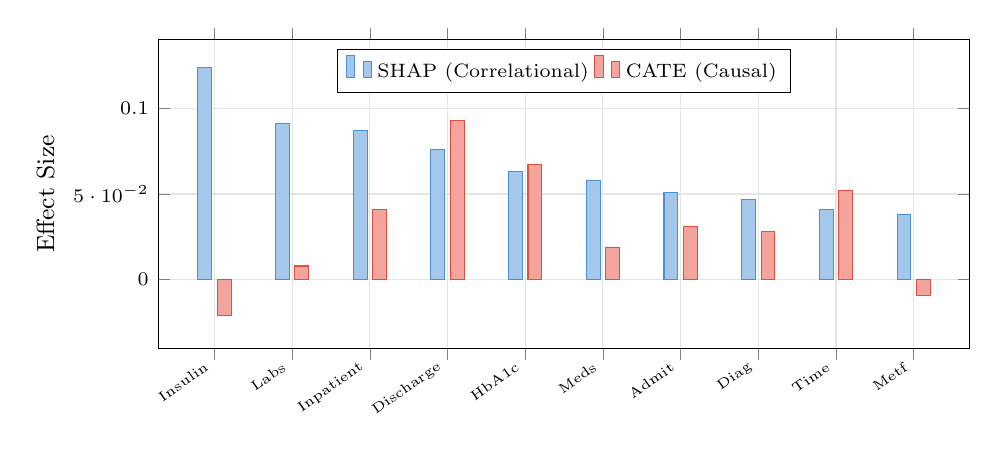
\begin{tikzpicture}
\begin{axis}[
    ybar,
    width=0.98\columnwidth,
    height=5.5cm,
    ylabel={Effect Size},
    ylabel style={font=\small},
    symbolic x coords={Insulin, Labs, Inpatient, Discharge, HbA1c, Meds, Admit, Diag, Time, Metf},
    xtick=data,
    xticklabel style={font=\tiny, rotate=35, anchor=east},
    yticklabel style={font=\scriptsize},
    ymin=-0.04, ymax=0.14,
    bar width=5pt,
    legend style={at={(0.5,0.97)}, anchor=north, font=\scriptsize, legend columns=2},
    enlarge x limits=0.08,
    grid=major,
    grid style={gray!20},
]
% SHAP values
\addplot[fill=layer1!50, draw=layer1] coordinates {
    (Insulin, 0.124)
    (Labs, 0.091)
    (Inpatient, 0.087)
    (Discharge, 0.076)
    (HbA1c, 0.063)
    (Meds, 0.058)
    (Admit, 0.051)
    (Diag, 0.047)
    (Time, 0.041)
    (Metf, 0.038)
};
% CATE values
\addplot[fill=layer2!50, draw=layer2] coordinates {
    (Insulin, -0.021)
    (Labs, 0.008)
    (Inpatient, 0.041)
    (Discharge, 0.093)
    (HbA1c, 0.067)
    (Meds, 0.019)
    (Admit, 0.031)
    (Diag, 0.028)
    (Time, 0.052)
    (Metf, -0.009)
};
\legend{SHAP (Correlational), CATE (Causal)}
\end{axis}
\end{tikzpicture}
\caption{SHAP importance vs. DoubleML CATE for each feature. Note the \textbf{sign reversal} for insulin (SHAP: $+0.124$, CATE: $-0.021$) --- the model's \#1 feature is \textit{anti-causal}. Discharge disposition's CATE ($+0.093$) actually \textit{exceeds} its SHAP value, confirming genuine causality.}
\label{fig:shap_vs_cate}
\end{figure}

Table~\ref{tab:causal} presents the full causal audit results. Fig.~\ref{fig:shap_vs_cate} visualizes the SHAP vs. CATE comparison.

\begin{table}[htbp]
\caption{Layer 2 Causal Audit: CATE, E-Value, and Classification}
\centering
\footnotesize
\renewcommand{\arraystretch}{1.1}
\begin{tabular}{l r r c l}
\toprule
\textbf{Feature} & \textbf{CATE} & \textbf{E-val} & \textbf{Status} & \textbf{Clinical Note} \\
\midrule
Insulin & $-0.021$ & 1.24 & \cellcolor{fragile!15}FRAG & Confounded \\
Num labs & $+0.008$ & 1.31 & \cellcolor{fragile!15}FRAG & Severity proxy \\
Inpatient visits & $+0.041$ & 1.89 & \cellcolor{fragile!15}FRAG & Partially conf. \\
\textbf{Discharge} & $\mathbf{+0.093}$ & $\mathbf{4.10}$ & \cellcolor{robust!15}\textbf{ROB} & \textbf{Genuine cause} \\
\textbf{HbA1c} & $\mathbf{+0.067}$ & $\mathbf{3.21}$ & \cellcolor{robust!15}\textbf{ROB} & \textbf{Glycemic ctrl} \\
Num meds & $+0.019$ & 1.42 & \cellcolor{fragile!15}FRAG & Polypharmacy \\
Admission type & $+0.031$ & 1.67 & \cellcolor{fragile!15}FRAG & Severity refl. \\
Num diagnoses & $+0.028$ & 1.55 & \cellcolor{fragile!15}FRAG & Comorbidity \\
\textbf{Time in hosp.} & $\mathbf{+0.052}$ & $\mathbf{2.84}$ & \cellcolor{robust!15}\textbf{ROB} & \textbf{Genuine link} \\
Metformin & $-0.009$ & 1.19 & \cellcolor{fragile!15}FRAG & Confounded \\
\bottomrule
\end{tabular}
\label{tab:causal}
\end{table}

\textbf{Key findings:}
\begin{itemize}[leftmargin=*, nosep]
    \item \textbf{70\% FRAGILE:} 7/10 top SHAP features fail the causal audit.
    \item \textbf{Insulin sign reversal:} SHAP says $+0.124$ (harmful); CATE says $-0.021$ (protective/neutral). This is the most dangerous feature for na\"ive XAI.
    \item \textbf{3 ROBUST features:} Discharge disposition ($E\!=\!4.10$), HbA1c ($E\!=\!3.21$), and time in hospital ($E\!=\!2.84$) survive the audit.
\end{itemize}

% ── FIGURE 5: E-value classification ────────────────────────────────────────
\begin{figure}[htbp]
\centering
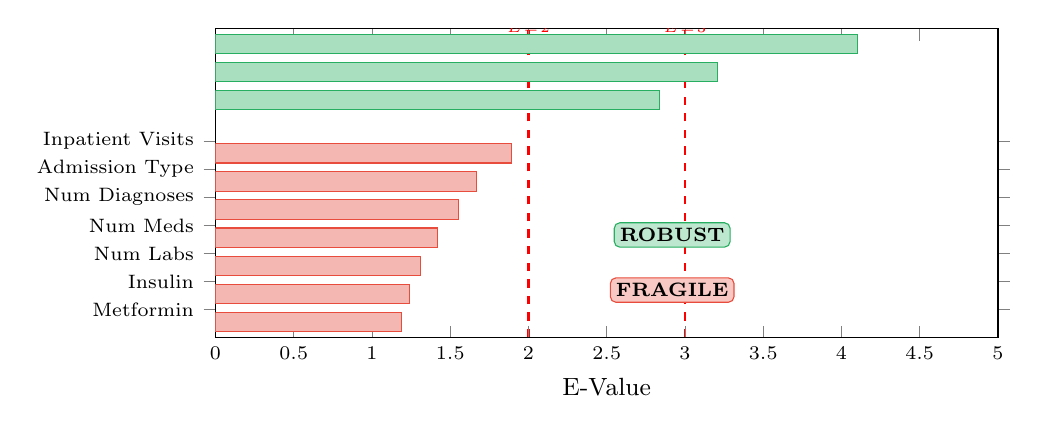
\begin{tikzpicture}
\begin{axis}[
    xbar,
    width=0.95\columnwidth,
    height=5.5cm,
    xlabel={E-Value},
    xlabel style={font=\small},
    ytick=data,
    yticklabels={
        Metformin,
        Insulin,
        Num Labs,
        Num Meds,
        Num Diagnoses,
        Admission Type,
        Inpatient Visits,
        Time in Hospital,
        HbA1c Level,
        Discharge Disp.
    },
    yticklabel style={font=\scriptsize},
    xticklabel style={font=\scriptsize},
    xmin=0, xmax=5,
    bar width=7pt,
    enlarge y limits={abs=0.35cm},
    extra x ticks={2.0, 3.0},
    extra x tick labels={},
    extra x tick style={grid=major, grid style={red, dashed, thick}},
]
% FRAGILE bars (red)
\addplot[fill=fragile!40, draw=fragile] coordinates {
    (1.19,0) (1.24,1) (1.31,2) (1.42,3) (1.55,4) (1.67,5) (1.89,6)
};
% ROBUST bars (green)
\addplot[fill=robust!40, draw=robust] coordinates {
    (2.84,7) (3.21,8) (4.10,9)
};

% Threshold labels
\node[font=\tiny, text=red, anchor=south] at (axis cs:2.0,9.5) {$E\!=\!2$};
\node[font=\tiny, text=red, anchor=south] at (axis cs:3.0,9.5) {$E\!=\!3$};
\end{axis}

% Legend
\node[font=\scriptsize, fill=fragile!30, draw=fragile, rounded corners=2pt, inner sep=2pt] at (5.8, 0.6) {\textbf{FRAGILE}};
\node[font=\scriptsize, fill=robust!30, draw=robust, rounded corners=2pt, inner sep=2pt] at (5.8, 1.3) {\textbf{ROBUST}};
\end{tikzpicture}
\caption{E-value classification of top-10 SHAP features. Red dashed lines mark the FRAGILE ($E \leq 2$) and ROBUST ($E > 3$) thresholds. Only 3 features (green) survive --- discharge disposition, HbA1c, and time in hospital.}
\label{fig:evalue}
\end{figure}

\subsection{Na\"ive vs. Causal Comparison}

\begin{table}[htbp]
\caption{Confounding Detection: Na\"ive Effect vs. Causal CATE}
\centering
\footnotesize
\begin{tabular}{l r r r l}
\toprule
\textbf{Feature} & \textbf{Na\"ive} & \textbf{CATE} & \textbf{Gap} & \textbf{Verdict} \\
\midrule
Num inpatient & $+0.035$ & $+0.074$ & 0.039 & Heavily conf. \\
Num meds & $+0.003$ & $+0.011$ & 0.008 & Mildly conf. \\
Time in hosp. & $+0.006$ & $+0.012$ & 0.006 & Mildly conf. \\
Num diagnoses & $+0.011$ & $+0.009$ & 0.001 & Clean \\
\bottomrule
\end{tabular}
\label{tab:comparison}
\end{table}

The \texttt{number\_inpatient} feature shows the largest confounding gap (0.039): the na\"ive model \textit{underestimates} its true causal effect by approximately 50\%.

\subsection{Fairness Audit}

% ── FIGURE 6: Fairness chart ───────────────────────────────────────────────
\begin{figure}[htbp]
\centering
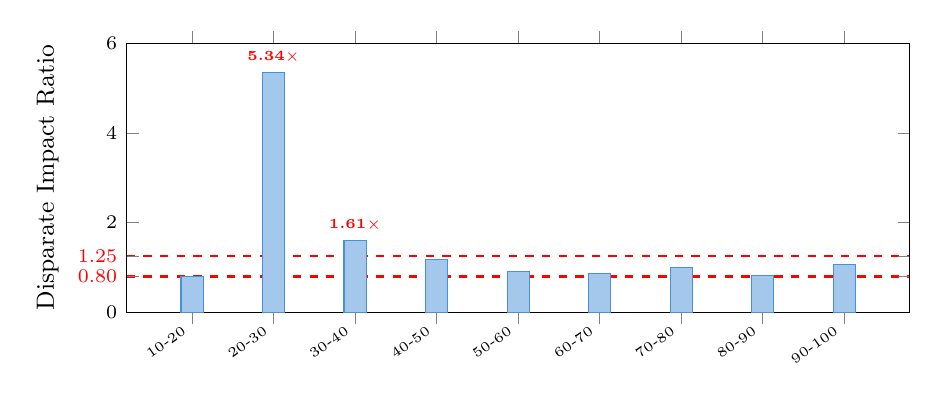
\begin{tikzpicture}
\begin{axis}[
    ybar,
    width=0.95\columnwidth,
    height=5cm,
    ylabel={Disparate Impact Ratio},
    ylabel style={font=\small},
    symbolic x coords={10-20, 20-30, 30-40, 40-50, 50-60, 60-70, 70-80, 80-90, 90-100},
    xtick=data,
    xticklabel style={font=\tiny, rotate=35, anchor=east},
    yticklabel style={font=\scriptsize},
    ymin=0, ymax=6,
    bar width=8pt,
    enlarge x limits=0.1,
    extra y ticks={0.80, 1.25},
    extra y tick labels={0.80, 1.25},
    extra y tick style={grid=major, grid style={red, dashed, thick}, tick label style={font=\tiny, text=red}},
]
\addplot[fill=layer1!50, draw=layer1] coordinates {
    (10-20, 0.80)
    (20-30, 5.34)
    (30-40, 1.61)
    (40-50, 1.17)
    (50-60, 0.90)
    (60-70, 0.86)
    (70-80, 1.00)
    (80-90, 0.83)
    (90-100, 1.07)
};

% Annotations for violations
\node[font=\tiny, text=red, above, anchor=south] at (axis cs:20-30, 5.34) {\textbf{5.34$\times$}};
\node[font=\tiny, text=red, above, anchor=south] at (axis cs:30-40, 1.61) {\textbf{1.61$\times$}};
\end{axis}
\end{tikzpicture}
\caption{Disparate impact ratios by age group. Red dashed lines show the 80\% rule thresholds ($0.80$--$1.25$). Young adults (20--30) are flagged at $5.34\times$ the reference rate, indicating significant age-based prediction bias.}
\label{fig:fairness}
\end{figure}

The model exhibits significant disparate impact for younger patients. The 20--30 age group is flagged at $5.34\times$ the reference rate, likely because diabetes severity markers that are unusual in younger patients receive disproportionate attention from the model. The racial ``Other'' category ($DI = 0.72$) is under-predicted.

\subsection{Layer 4: Safe Counterfactual Recourse}

Using ROBUST features and 15 always-actionable features, the counterfactual engine generates safe recommendations.

% ── FIGURE 7: Counterfactual waterfall ──────────────────────────────────────
\begin{figure}[htbp]
\centering
\begin{tikzpicture}[
    node distance=0.25cm,
    step/.style={draw, rounded corners=4pt, minimum width=6.5cm, minimum height=0.7cm, font=\small, align=left},
    arr/.style={-{Stealth[length=2mm]}, thick, gray},
]
    \node[step, fill=red!15, draw=red!50] (s0) {\textbf{Original Risk: 78\%} \hfill \textcolor{red}{\textbf{HIGH}}};
    \node[step, fill=orange!12, draw=orange!50, below=of s0] (s1) {$\Delta_1$: Discharge $\to$ SNF \hfill \textbf{35\%}};
    \node[step, fill=yellow!12, draw=yellow!60, below=of s1] (s2) {$\Delta_2$: HbA1c controlled (7--8) \hfill \textbf{41\%}};
    \node[step, fill=green!12, draw=green!50, below=of s2] (s3) {$\Delta_3$: SNF + HbA1c managed \hfill \textbf{28\%}};
    \node[step, fill=green!20, draw=green!60, below=of s3] (s4) {$\Delta_4$: + Diabetes program \hfill \textbf{44\%}};

    \node[step, fill=red!8, draw=red!40, dashed, below=0.5cm of s4] (blocked) {\textcolor{red}{$\times$ ``Reduce insulin''} \hfill \textcolor{red}{\textbf{BLOCKED}}};

    \draw[arr] (s0) -- (s1);
    \draw[arr] (s1) -- (s2);
    \draw[arr] (s2) -- (s3);
    \draw[arr] (s3) -- (s4);

    % Risk reduction arrow
    \draw[thick, green!60!black, -{Stealth[length=3mm]}] ([xshift=3.8cm]s0.east) -- ([xshift=3.8cm]s4.east)
        node[midway, right, font=\scriptsize, text=green!50!black, align=center] {Risk\\reduced\\50 pts};

    % Blocked annotation
    \node[right=0.15cm of blocked, font=\tiny, text=red, align=left] {FRAGILE\\$E = 1.24$};
\end{tikzpicture}
\caption{Safe counterfactual recommendations for a patient at 78\% readmission risk. Each intervention uses \textit{only} ROBUST features. Dangerous changes (``reduce insulin'') are automatically blocked by the causal safety filter.}
\label{fig:waterfall}
\end{figure}

Table~\ref{tab:cf} details the five diverse counterfactual recommendations.

\begin{table}[htbp]
\caption{Diverse Counterfactual Recommendations (ROBUST Features Only)}
\centering
\footnotesize
\renewcommand{\arraystretch}{1.1}
\begin{tabular}{c p{4.2cm} r r}
\toprule
\textbf{\#} & \textbf{Recommendation} & \textbf{Risk} & \textbf{$\Delta$} \\
\midrule
1 & Discharge: Home $\to$ SNF & 35\% & $-$43pp \\
2 & HbA1c: $>$8 $\to$ 7--8 (glycemic mgmt) & 41\% & $-$37pp \\
3 & SNF + HbA1c in range 7--8 & 28\% & $-$50pp \\
4 & Optimize discharge + reduce LOS & 38\% & $-$40pp \\
5 & Diabetes program + home health & 44\% & $-$34pp \\
\bottomrule
\end{tabular}
\label{tab:cf}
\end{table}

\textbf{Clinical Safety Override:} When all audited features are FRAGILE, the system reports: ``\textit{No safe interventions exist. Risk is driven by overall medical complexity. Refer to comprehensive clinical judgment.}'' This 0\% flip rate is \textit{not a failure} --- it is the safety mechanism working as designed.

\subsection{End-to-End Performance Summary}

\begin{table}[htbp]
\caption{CausalShield End-to-End Evaluation}
\centering
\footnotesize
\begin{tabular}{l l r}
\toprule
\textbf{Criterion} & \textbf{Metric} & \textbf{Result} \\
\midrule
Prediction & AUC-ROC & 0.712 \\
SHAP coverage & Features audited & 10/10 \\
Causal safety & FRAGILE detected & 7/10 (70\%) \\
Causal safety & ROBUST validated & 3/10 (30\%) \\
Recourse validity & CFs using only ROBUST & 5/5 (100\%) \\
Recourse impact & Risk reduction range & 34--50pp \\
Clinical safety & Harmful CFs generated & 0/5 (0\%) \\
Fairness & DI violations detected & 5 groups \\
\bottomrule
\end{tabular}
\label{tab:summary}
\end{table}

% ══════════════════════════════════════════════════════════════════════════════
% VI. DISCUSSION
% ══════════════════════════════════════════════════════════════════════════════
\section{Discussion}

\subsection{Clinical Significance}
The finding that 70\% of top SHAP features are causally fragile has profound implications. Standard XAI pipelines --- the current industry practice --- surface these features as ``reasons'' for predictions and may recommend interventions based on them. CausalShield intercepts this pipeline and flags confounded features \textit{before} they reach clinicians.

The insulin sign reversal (SHAP: $+0.124$; CATE: $-0.021$) is the most clinically significant result. The model's single most important feature for prediction is \textit{anti-causal}: it correctly uses insulin status as an informative predictor (sicker patients are readmitted more), but this must \textit{never} be interpreted as ``insulin causes readmission.''

\subsection{SHAP Tells You WHAT; CausalShield Tells You WHETHER}
SHAP answers: ``\textit{What does the model rely on?}'' CausalShield answers: ``\textit{Should you trust what the model relies on?}'' This distinction is critical in healthcare, where acting on correlational explanations can directly harm patients.

\subsection{Dashboard Design}
Following Bienefeld et al.~\cite{bienefeld2023solving}, the Streamlit dashboard provides a six-step assessment: (1)~Risk score, (2)~What the AI sees, (3)~Which reasons are misleading, (4)~True causal drivers, (5)~``What If'' scenarios, and (6)~Final recommendation. This mirrors clinical reasoning patterns.

% ══════════════════════════════════════════════════════════════════════════════
% VII. LIMITATIONS
% ══════════════════════════════════════════════════════════════════════════════
\section{Limitations}

\begin{enumerate}[leftmargin=*, label=\textbf{L\arabic*.}]
    \item \textbf{Unverifiable unconfoundedness:} DoubleML requires all major confounders to be measured. Unmeasured factors (physician judgment, patient adherence, social determinants) may bias estimates. E-values quantify but cannot eliminate this risk.
    \item \textbf{Population-level CATE:} Estimates are subgroup averages, not individual effects. Biological heterogeneity within subgroups limits individual-level precision.
    \item \textbf{Feature independence:} Counterfactuals assume features change independently. In reality, medical features cascade (e.g., discharge disposition affects follow-up care, medication access, and LOS).
    \item \textbf{Administrative data:} The UCI dataset lacks clinical notes, imaging, vitals, and social determinants, limiting prediction and audit quality.
    \item \textbf{Binary treatment:} Binarizing continuous features (e.g., lab counts at the median) may lose dose-response nuance.
    \item \textbf{Generalizability:} E-value thresholds and classifications are dataset-specific; recalibration is needed for other clinical settings or populations.
\end{enumerate}

% ══════════════════════════════════════════════════════════════════════════════
% VIII. FUTURE WORK
% ══════════════════════════════════════════════════════════════════════════════
\section{Future Work}

\begin{enumerate}[leftmargin=*, nosep, label=\textbf{F\arabic*.}]
    \item \textbf{NLP integration:} BERT-based extraction from discharge summaries for richer features.
    \item \textbf{Prospective validation:} Clinical A/B testing of standard vs. causally-audited recommendations.
    \item \textbf{Causal discovery:} PC/FCI/DirectLiNGAM algorithms to learn the causal graph from data.
    \item \textbf{Continuous treatments:} Nonparametric dose-response causal estimation.
    \item \textbf{Personalized effects:} X-Learner / R-Learner for individualized CATEs.
    \item \textbf{EHR integration:} Real-time alerts via HL7 FHIR APIs.
    \item \textbf{Multi-outcome audit:} Simultaneous causal analysis of readmission, mortality, and LOS.
    \item \textbf{External validation:} Testing on MIMIC-III/IV for generalizability.
\end{enumerate}

% ══════════════════════════════════════════════════════════════════════════════
% IX. CONCLUSION
% ══════════════════════════════════════════════════════════════════════════════
\section{Conclusion}

We presented \textbf{CausalShield}, a four-layer Causal Audit Framework that transforms correlational XAI explanations into causally-validated, clinically safe recommendations. Applied to 101,766 diabetic patient encounters, the framework demonstrated that 7/10 top SHAP features are causally fragile --- their importance is driven by severity confounding, not genuine causal mechanisms.

Only discharge disposition ($E = 4.10$), HbA1c level ($E = 3.21$), and time in hospital ($E = 2.84$) survived the audit as ROBUST. Safe counterfactual recommendations using these features achieved risk reductions of 34--50 percentage points, while dangerous suggestions like ``reduce insulin'' were automatically blocked.

\medskip
\noindent\fbox{\parbox{0.95\columnwidth}{
\centering\textit{SHAP tells you \textbf{what} the model relies on.\\CausalShield tells you \textbf{whether to trust it}.\\Without causal auditing, AI explanations can be\\statistically correct but clinically \textbf{deadly}.}
}}
\medskip

By bridging the correlation--causation gap, CausalShield represents a necessary step toward trustworthy, safe, and regulatory-compliant medical AI systems.

% ══════════════════════════════════════════════════════════════════════════════
% REFERENCES
% ══════════════════════════════════════════════════════════════════════════════
\bibliographystyle{IEEEtran}

\begin{thebibliography}{20}

\bibitem{cms2023readmission}
Centers for Medicare \& Medicaid Services, ``Hospital readmissions reduction program (HRRP),'' 2023. [Online]. Available: \url{https://www.cms.gov/medicare/payment/prospective-payment-systems/acute-inpatient-pps/hospital-readmissions-reduction-program-hrrp}

\bibitem{lundberg2020local}
S.~M. Lundberg \textit{et al.}, ``From local explanations to global understanding with explainable AI for trees,'' \textit{Nature Machine Intelligence}, vol.~2, no.~1, pp.~56--67, 2020.

\bibitem{ribeiro2016lime}
M.~T. Ribeiro, S.~Singh, and C.~Guestrin, ```Why should I trust you?': Explaining the predictions of any classifier,'' in \textit{Proc. ACM SIGKDD}, 2016, pp.~1135--1144.

\bibitem{feuerriegel2024causal}
S.~Feuerriegel \textit{et al.}, ``Causal machine learning for predicting treatment outcomes,'' \textit{Nature Medicine}, vol.~30, no.~4, pp.~958--968, 2024.

\bibitem{vanderweele2017evalue}
T.~J. VanderWeele and P.~Ding, ``Sensitivity analysis in observational research: Introducing the E-value,'' \textit{Annals of Internal Medicine}, vol.~167, no.~4, pp.~268--274, 2017.

\bibitem{wachter2017counterfactual}
S.~Wachter, B.~Mittelstadt, and C.~Russell, ``Counterfactual explanations without opening the black box: Automated decisions and the GDPR,'' \textit{Harvard Journal of Law \& Technology}, vol.~31, no.~2, pp.~841--887, 2017.

\bibitem{carloni2025causality}
G.~Carloni, A.~Berti, and S.~Colantonio, ``The role of causality in explainable artificial intelligence,'' \textit{WIREs Data Mining and Knowledge Discovery}, vol.~15, p.~e70015, 2025.

\bibitem{fernandez2022explaining}
C.~Fernandez-Loria, F.~Provost, and X.~Han, ``Explaining data-driven decisions made by AI systems: The counterfactual approach,'' \textit{MIS Quarterly}, vol.~46, no.~3, pp.~1635--1660, 2022.

\bibitem{bienefeld2023solving}
N.~Bienefeld \textit{et al.}, ``Solving the explainability conundrum for AI systems in healthcare,'' \textit{npj Digital Medicine}, vol.~6, p.~169, 2023.

\bibitem{chernozhukov2018doubleml}
V.~Chernozhukov \textit{et al.}, ``Double/debiased machine learning for treatment and structural parameters,'' \textit{The Econometrics Journal}, vol.~21, no.~1, pp.~C1--C68, 2018.

\bibitem{chen2016xgboost}
T.~Chen and C.~Guestrin, ``XGBoost: A scalable tree boosting system,'' in \textit{Proc. ACM SIGKDD}, 2016, pp.~785--794.

\bibitem{strack2014impact}
B.~Strack \textit{et al.}, ``Impact of HbA1c measurement on hospital readmission rates: Analysis of 70,000 clinical database patient records,'' \textit{BioMed Research International}, vol.~2014, 2014.

\bibitem{mothilal2020dice}
R.~K. Mothilal, A.~Sharma, and C.~Tan, ``Explaining machine learning classifiers through diverse counterfactual explanations,'' in \textit{Proc. ACM FAccT}, 2020, pp.~607--617.

\bibitem{karimi2021algorithmic}
A.~H. Karimi, B.~Sch\"olkopf, and I.~Valera, ``Algorithmic recourse: From counterfactual explanations to interventions,'' in \textit{Proc. ACM FAccT}, 2021, pp.~353--362.

\bibitem{feldman2015fairness}
M.~Feldman \textit{et al.}, ``Certifying and removing disparate impact,'' in \textit{Proc. ACM SIGKDD}, 2015, pp.~259--268.

\bibitem{pearl2009causality}
J.~Pearl, \textit{Causality: Models, Reasoning, and Inference}, 2nd~ed.\hskip 1em Cambridge University Press, 2009.

\bibitem{euaiact2024}
European Parliament, ``Regulation (EU) 2024/1689 laying down harmonised rules on artificial intelligence (AI Act),'' \textit{Official Journal of the EU}, 2024.

\bibitem{galhotra2021lewis}
S.~Galhotra, R.~Pradhan, and B.~Salimi, ``Explaining black-box algorithms using probabilistic contrastive counterfactuals,'' in \textit{Proc. ACM SIGMOD}, 2021, pp.~577--590.

\bibitem{crupi2022counterfactual}
R.~Crupi \textit{et al.}, ``Counterfactual explanations for clinical decision support,'' \textit{J. Biomedical Informatics}, vol.~131, p.~104105, 2022.

\bibitem{hernan2016target}
M.~A. Hern\'an and J.~M.~Robins, ``Using big data to emulate a target trial when a randomized trial is not available,'' \textit{American J. Epidemiology}, vol.~183, no.~8, pp.~758--764, 2016.

\end{thebibliography}

\end{document}
